\section{Исследовательский раздел}

В данном разделе проведено исследование эффективности и применимости разработанного программного обеспечения. Выполнено сравнение результатов работы разработанного метода и метода с аппаратной поддержкой доверенной среды исполнения на базе процессоров с архитектурой ARM (ARM TrustZone).

\subsection{Методика проведения исследования}

Для того чтобы иследовать эффективность и применимость разработанного программного обеспечения, необходимо сравнить количество машинных инструкций для выполнения задач ДСИ: смена контекста между мирами, проверка целостности, обработку прерываний и так далее. Для точного подсчета количества выполняемых инструкций за промежуток времени, был использовано аппаратное расширение ARM Performance Monitoring Unit \cite{arm-performance-monitor}. Было подсчитано количество инструкций для выполнения одинаковых задач с использованием виртуализации ARM TrustZone и аппаратного решения.

В качестве ядра гостевой ОС был использовано ядро Linux версии 6.15, а в качестве ядра привилегированной ОС --- OP-TEE версии 4.0. В качестве гипервизора был использован KVM, который является частью ядра Linux.

Сравнение было проведено как для 32-битных процессоров с архитектурой ARMv7 так и для более новых, 64-битных процессоров с архитектурой ARMv8. Были выбраны два устройства: Raspberry Pi 4 Model B \cite{rpi4-b} и Raspberry Pi 2 Model \cite{rpi2-b}. Raspberry Pi 4 Model B обладает следующими характеристиками:

\begin{itemize}
	\item [---] 4 64-битных ядра Cortex A72 (ARMv8) с тактовой частотой 1,5Ггц.
	\item [---] 8 Гб ОЗУ.
\end{itemize}

Raspberry Pi 2 обладает следующими характеристиками:

\begin{itemize}
	\item [---] 4 32-битных ядра Cortex A7 (ARMv7) с тактовой частотой 0.9ГГц.
	\item [---] 1 Гб ОЗУ.
\end{itemize}

Во время проведения исследования для каждой виртуальной машины было выделен 1 виртуальный CPU который соотвествует 1 физическому CPU.

\subsection{Сравнение количества машинных инструкций с аппаратной реализацией} 

\subsubsection{Сравнение при выполнение ключевых задач}

Можно выделить три ключевые задачи, выполняемых доверенной средой исполнения, без которых она не может считаться полноценной:

\begin{enumerate}[label*=\arabic*.]
	\item смена контекста выполнения между гостевым и доверенным миром;
	\item разделение аппаратных ресурсов;
	\item проверка целостности загружаемых образов ОС.
\end{enumerate}

В таблице \ref{table:perf-main-1} представлено сравнение количества машинных инструкций для смены контекста выполнения и разделения аппаратных ресурсов между мирами: разделение памяти и прерываний. В первых двух столбцах указаны результаты сравнения на устройстве Raspberry Pi 2 Model B; первый столбец --- аппаратная реализация, второй --- визуализация (разработанный метод). В третьем и четвертом столбце указанные результаты сравнения выполняемые на устройстве Raspberry Pi 4 Model, для аппаратной и виртуализированной реализации соответственно.

\begin{table}[!htb]
	\begin{center}
		\caption{Сравнение количества инструкций необходимых для выполнения ключевых задач ДСИ}
		\label{table:perf-main-1}
		\begin{tabular}{|c|c|c|c|c|}
			\hline
			& \bfseries R Pi2 (А) & \bfseries R Pi2 (В) & \bfseries R Pi4 (А) & \bfseries R Pi4 (В)\\
			\hline
			\bfseries Смена контекста & 9200 & 18745 & 1525 & 7625 \\ \hline
			\bfseries Разделение участков памяти & 3245 & 7055 & 2208 & 7800 \\ \hline
			\bfseries Разделение прерываний & 2273 & 6251 & 986 & 3421 \\ \hline	
		\end{tabular}
	\end{center}
\end{table}

По результатам из таблицы \ref{table:perf-main-1} можно сделать вывод, что смена контекста для 32-битных процессоров в разработанном методе требует в два раза больше инструкций, чем в аппаратной реализации ARM TrustZone. Для 64-битных процессоров разница составляет порядка 5 раз. Данную разницу можно счесть приемлемой, так как смена контекста между мирами происходит редко и практически никак не отражается на производительности выполняемых приложений и всей системы в целом.

Для выполнения разделения участков памяти, по сравнению с аппаратной реализацией, необходимо в 2 и 4 раза для 32-битных и 64-битных процессоров соответственно. Для разделения и корректной маршрутизации прерываний необходимо в 3 раза больше инструкций как для 32-битных, так и для 64-битных процессоров. Данную разницу, так же, как и в случае со сменой контекста, можно счесть приемлемой, так как операции разделения ресурсов выполняются редко.

В таблице \ref{table:perf-main-2} представлено сравнение количества машинных инструкций для проверки целостности загружаемых образов ОС. Для этого было проведено хеширование регионов памяти размером 1, 16, 32, 64 и 128 Кб с помощью алгоритма SHA256 \cite{sha-256}.

\begin{table}[!htb]
	\begin{center}
		\caption{Сравнение количества инструкций необходимых для выполнения проверки целостности}
		\label{table:perf-main-2}
		\begin{tabular}{|c|c|c|c|c|}
			\hline
			& \bfseries R Pi2 (А) & \bfseries R Pi2 (В) & \bfseries R Pi4 (А) & \bfseries R Pi4 (В)\\
			\hline
			\bfseries 1 Кб & 1150 & 1256 & 300 & 325 \\ \hline
			\bfseries 16 Кб & 17890 & 19200 & 4450 & 4800 \\ \hline
			\bfseries 32 Кб  & 36502 & 38600 & 10200 & 11223 \\ \hline	
			\bfseries 64 Кб  & 80215 & 84555 & 22254 & 23507 \\ \hline	
			\bfseries 128 Кб  & 165865 & 170205 & 50700 & 51998 \\ \hline	
		\end{tabular}
	\end{center}
\end{table}

По результатам из таблицы \ref{table:perf-main-2}, можно сделать вывод что накладные расходы для выполнения проверки целостности в среднем составляют 5-10\% по сравнению с аппаратной реализацией, что не является критичным и не влияет на производительность системы.

\subsubsection{Сравнение с использованием пользовательских приложений}

Для сравнения накладных ресурсов при использовании пользовательских приложений были выбраны приложения ccrypt и GoHttp. ccrypt был использован для шифрования файлов размеров 1 Кб, а GoHttp для передачи по сети. Логика шифрования данных реализована на уровне доверенной среды исполнения. 

Было проведено сравнение количества выполняемых как и с одной парой (гостевая и доверенная ОС) виртуальных машин, так и при запуске нескольких пар одновременно.

На рисунках \ref{fig:perf-user-1-armv7} и \ref{fig:perf-user-1-armv8} представлено сравнение (в процентах) количества используемых инструкций при использовании одной пары ВМ. Аппаратная реализция отмечена как 100\%.

\begin{figure}[h]
	\centering
	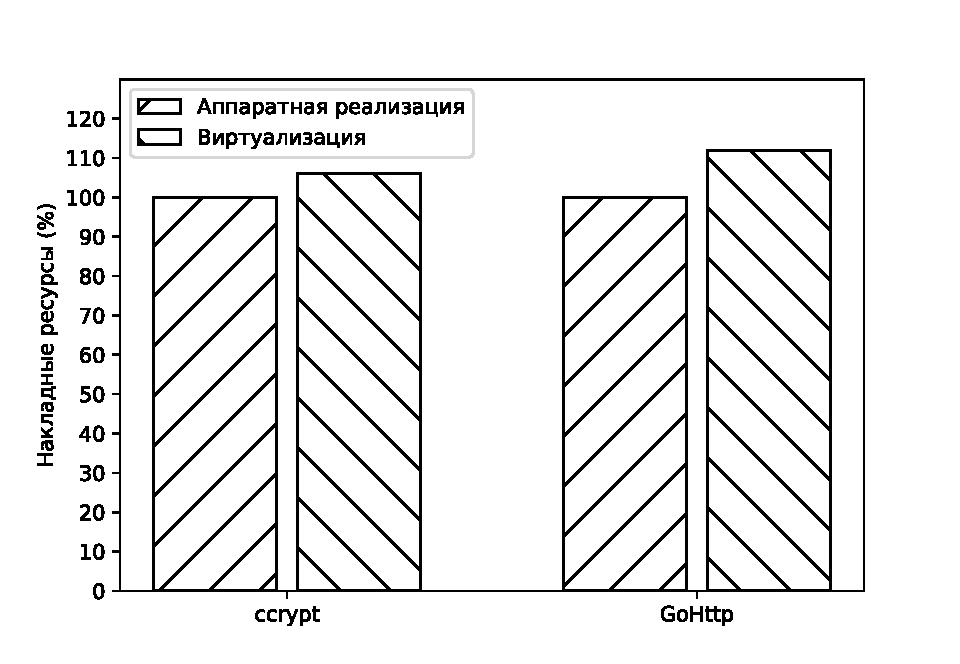
\includegraphics[width=\textwidth]{img/user-1-armv7.pdf}
	\caption{Сравнение результатов выполнения пользовательских приложений (ARMv7)}
	\label{fig:perf-user-1-armv7}
\end{figure}

\begin{figure}[h]
	\centering
	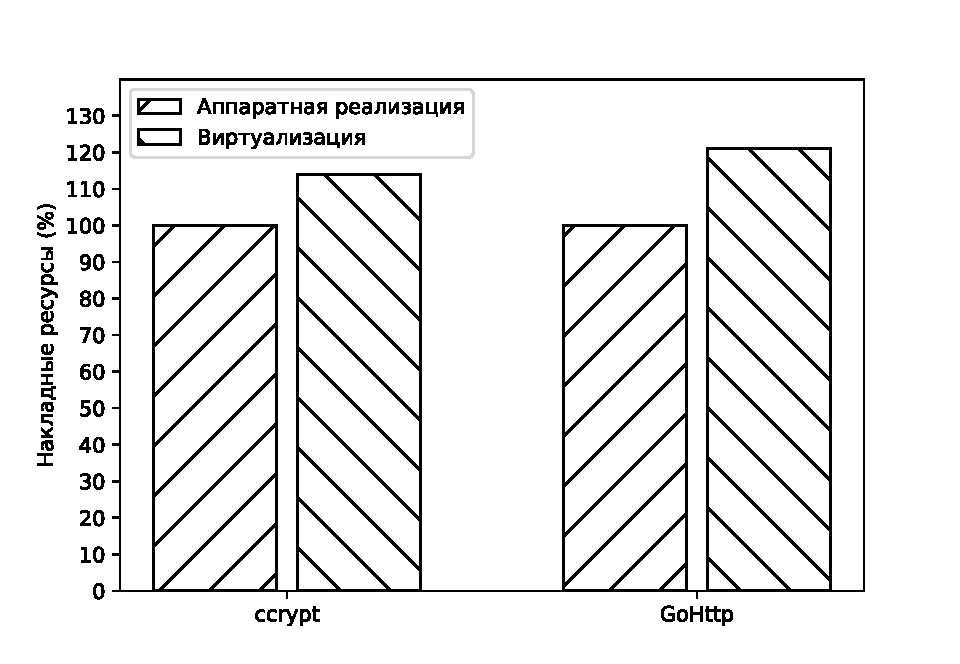
\includegraphics[width=\textwidth]{img/user-1-armv8.pdf}
	\caption{Сравнение результатов выполнения пользовательских приложений (ARMv8)}
	\label{fig:perf-user-1-armv8}
\end{figure}

На рисунках \ref{fig:perf-user-2-armv7} и \ref{fig:perf-user-2-armv8} представлено сравнение количества инструкций при использовании нескольких пар ВМ, которые передают файлы размером 1Кб между друг другом с использованием приложения GoHTTP.

\begin{figure}[h]
	\centering
	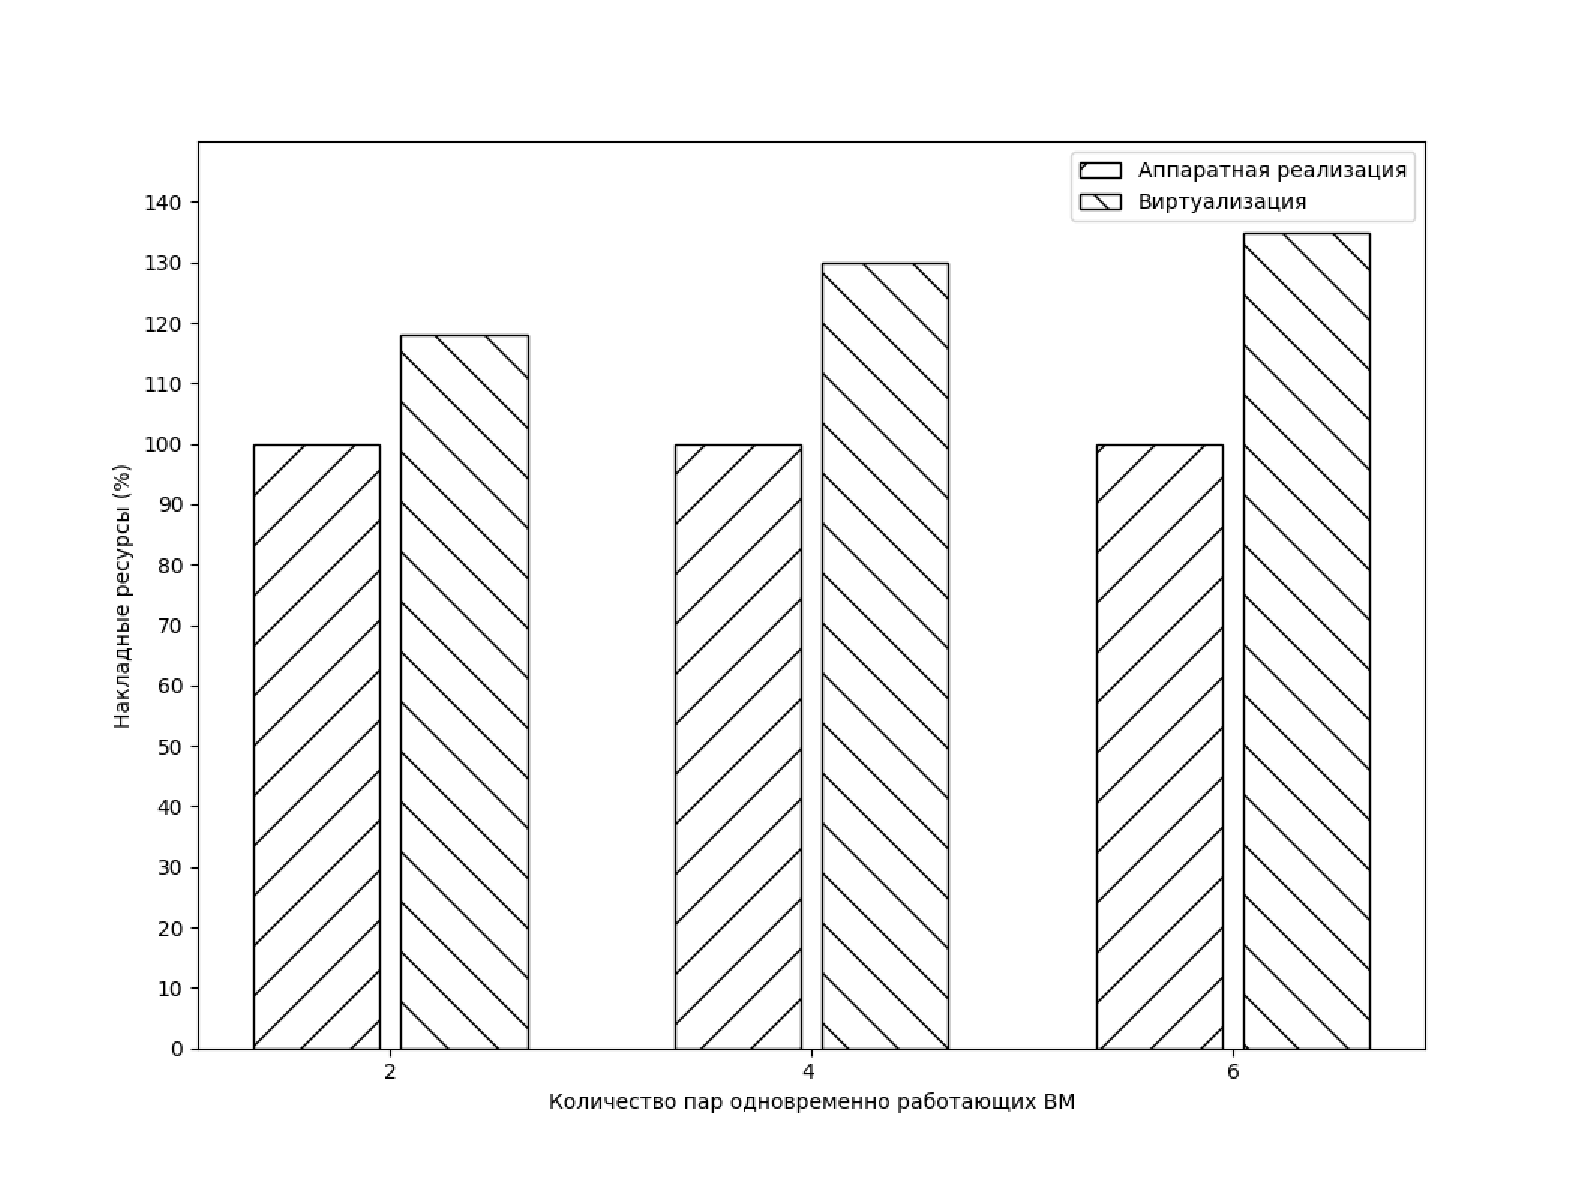
\includegraphics[width=\textwidth]{img/user-2-armv7.pdf}
	\caption{Сравнение результатов выполнения пользовательских приложений (ARMv7), несколько пар ВМ}
	\label{fig:perf-user-2-armv7}
\end{figure}

\begin{figure}[h]
	\centering
	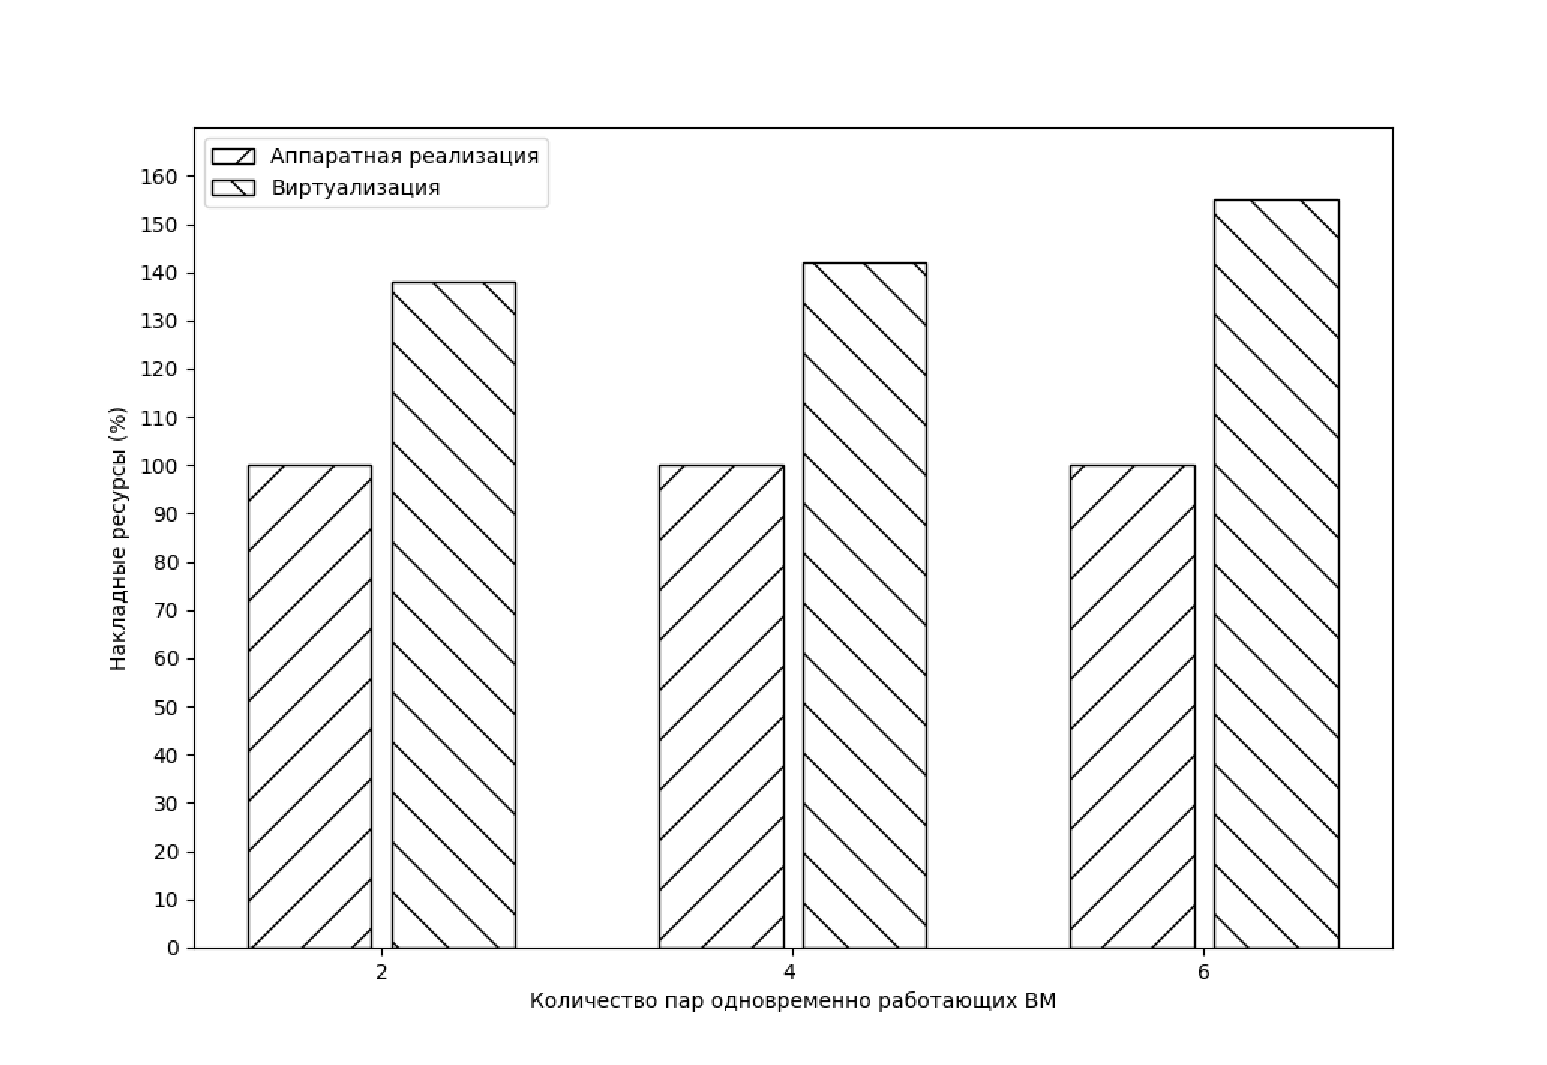
\includegraphics[width=\textwidth]{img/user-2-armv8.pdf}
	\caption{Сравнение результатов выполнения пользовательских приложений (ARMv8), несколько пар ВМ}
	\label{fig:perf-user-2-armv8}
\end{figure}

Можно сделать вывод, что при использовании одной пары ВМ, накладные ресурсы на исполнение пользовательских приложений в среднем составляют 7-15\%. При использовании нескольких пар ВМ, накладные ресурсы возрастают и составляют от 20 до 50\% по сравнению с аппаратной реализацией. Заметный рост накладных ресурсов наблюдается при использовании двух пар ВМ (20\% и 35\% для ARMv7 и ARMv8 соответственно), но незначительный рост в 5-10\% при увеличении количества пар (две и более). Можно сделать вывод, что ключевую роль в увеличении накладных расходов играет тот факт, что параллельно используется более одной пары ВМ, а не зависит от их количества: разница при использовании 2 и 6 пара ВМ составляет 7-15\%.

\subsubsection{Сравнение с использованием серверных приложений}

Для тестирования накладных ресурсов при использовании серверных приложений были выбраны MongoDB \cite{mongodb} и Apache \cite{apache}. Количество виртуальных CPU для каждой ВМ было увеличено до 4. Используется одна пара ВМ. В качестве устройства использовался Raspberry Pi 4 Model B (ARMv8).

На рисунке \ref{fig:system-1} представлены результаты сравнения с использованием\\MongoDB: клиент, расположенный на той же ВМ, что и сервер, на протяжении 1 минуты вставляет объекты различного размера в таблицу базы данных. 

\begin{figure}[h]
	\centering
	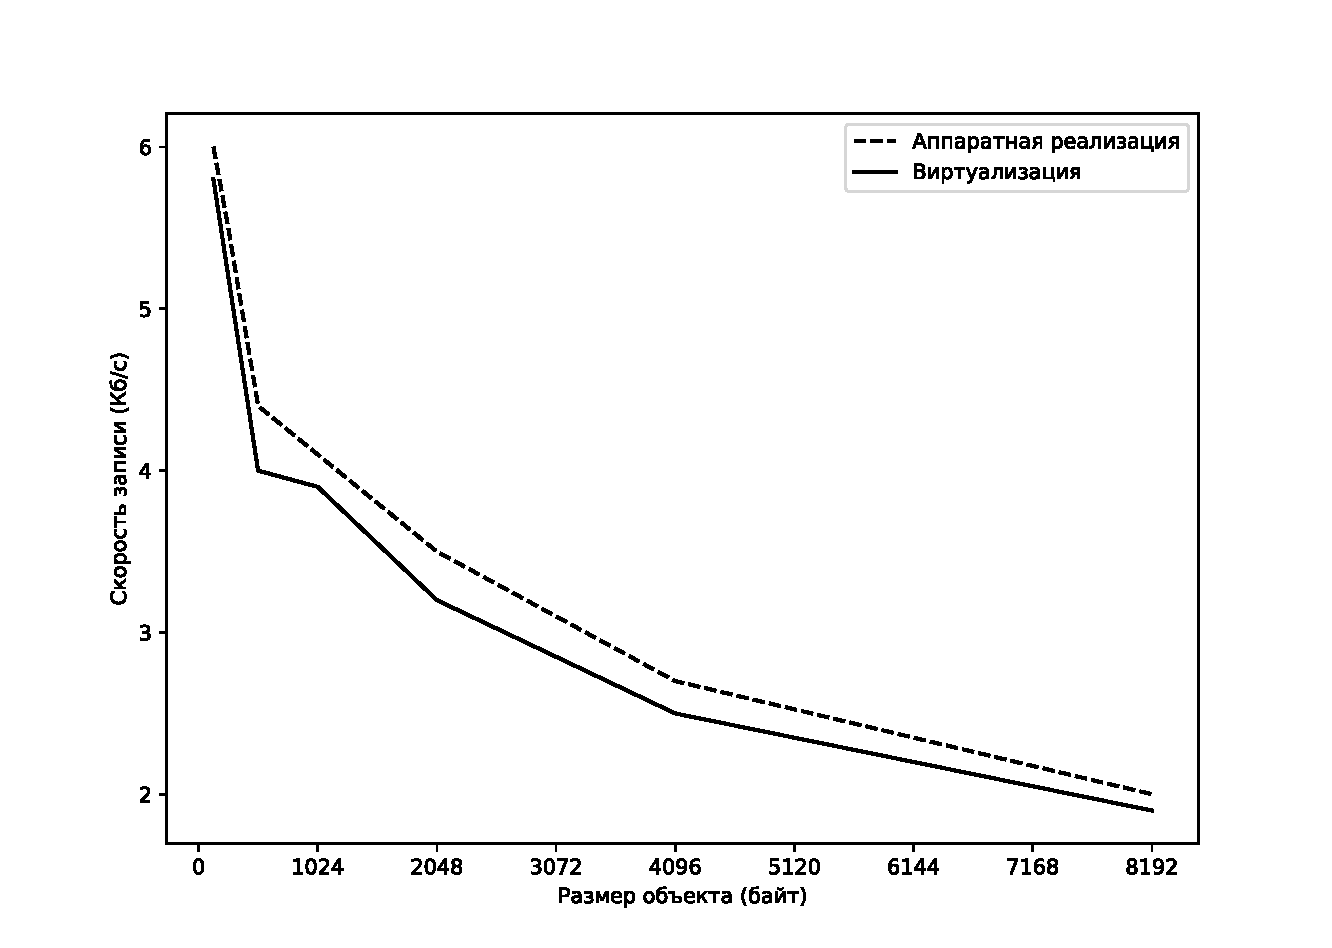
\includegraphics[width=\textwidth]{img/system-1.pdf}
	\caption{Зависимость скорости записи на сервер MongoDB от размера объекта}
	\label{fig:system-1}
\end{figure}

Из риснука \ref{fig:system-1} можно сделать вывод о том, что при использовании разработанного метода скорость записи в сервер MongoDB практически идентична скорости записи при использовании аппаратного метода: разница составляет 5-10\%.

На рисунке \ref{fig:system-2} представлены результаты сравнения с использованием\\Apache: клиент, расположенный на той же ВМ, что и сервер, на протяжении 1 минуты скачивает файл различного размера с сервера.

\begin{figure}[h]
	\centering
	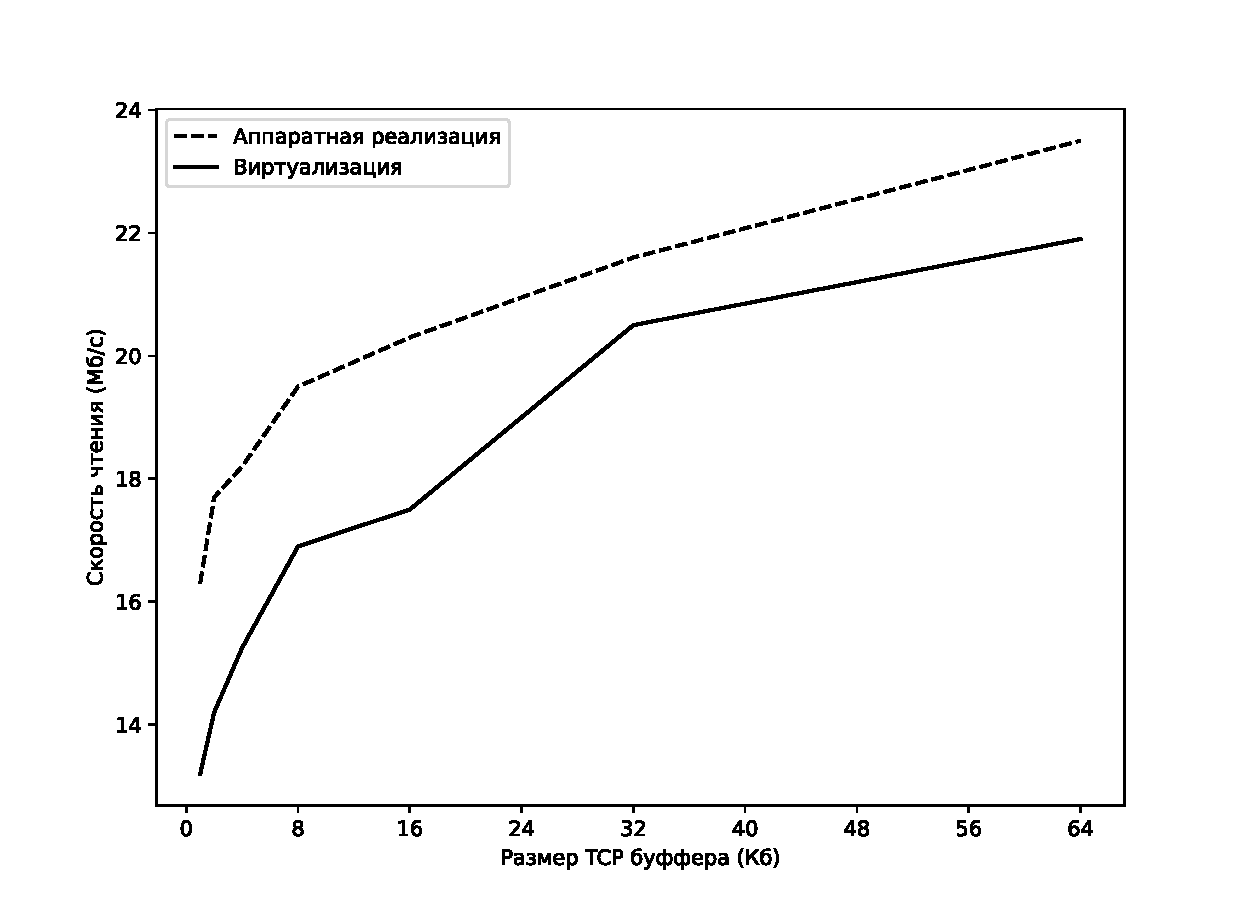
\includegraphics[width=\textwidth]{img/system-2.pdf}
	\caption{Зависимость скорости чтения данных с сервера Apache от размера TCP буффера}
	\label{fig:system-2}
\end{figure}

Из рисунка \ref{fig:system-1} можно так же сделать вывод, что скорость чтения с сервера Apache при использовании разработанного метода близка к скорости с использованием аппаратной реализации: разница составляет 10-15\%.

\subsection*{Вывод}

В данном разделе проведено исследование эффективности разработанного программного обеспечения. Было произведено сравнение количества используемых машинных инструкций для выполнения ключевых задач ДСИ: 

\begin{itemize}
	\item [---] Для смены контекста требуется в 2 и 5 раз больше инструкций для 32-битных (ARMv7) и 64-битных (ARMv8) процессоров соотвественно.
	\item [---] Для обработки разделения аппаратных ресурсов в среднем требуется в 2-4 раза больше инструкций.
	\item [---] Разница в количестве инструкций для проверки целостности образов ОС между разработанным методом и аппаратной реализацией в среднем составляет 5-10\%.
\end{itemize}

Во всех приведенных сравнениях, для 32-битных процессоров разница в количестве инструкций составляет меньше, чем для 64-битных (в среднем в 1.5-2 раза). 

Произведено сравнение накладных ресурсов при использовании пользовательских и серверных приложений.

\begin{itemize}
	\item [---] Для пользовательских приложений разница с аппаратной реализацией составляет 7-15\% и 20-50\% при использовании нескольких виртуальных машин одновременно.
	\item [---] Накладные расходы резко возрастают (на 20-40\%) если в системе используется более одной пары ВМ.
	\item [---] Произведено сравнение скорости записи данных в сервер MongoDB: разница с аппаратной реализацией составляет 5-10 в зависимости от размера данных\%.
	\item [---] При чтении файлов с сервера Apache было установлено, что скорость чтения на 10-15\% меньше, чем при использовании аппаратной реализации.
\end{itemize}

\pagebreak
